% Template for ICASSP-2018 paper; to be used with:
%          spconf.sty  - ICASSP/ICIP LaTeX style file, and
%          IEEEbib.bst - IEEE bibliography style file.
% --------------------------------------------------------------------------
\documentclass{article}
\usepackage{spconf,amsmath,amssymb,graphicx,bm}
\graphicspath{{figures/}}

\newcommand{\R}{\mathbb{R}}
\renewcommand{\vec}[1]{\ensuremath{\mathbf{#1}}}
\providecommand{\mat}[1]{\ensuremath{\mathbf{#1}}}
\providecommand{\vx}{\vec{x}}
\providecommand{\vy}{\vec{y}}
\providecommand{\ve}{\vec{e}}
\providecommand{\vn}{\vec{n}}
\providecommand{\vA}{\vec{A}}
\providecommand{\norm}[1]{\left\lVert#1\right\rVert}
\DeclareMathOperator*{\argmin}{arg\,min}
\DeclareMathOperator*{\argmax}{arg\,max}

\title{Optimal Measurement Configuration in Computational \\ Multispectral Imaging With a Diffractive Lens}

\name{Evan Widloski \qquad Ulas Kamaci \qquad Farzad Kamalabadi}
\address{
Department of Electrical and Computer Engineering and Coordinated Science Laboratory, \\
University of Illinois at Urbana-Champaign, Urbana, IL 61801, USA
}

\begin{document}
\maketitle

\begin{abstract}
% Spectral imaging, forming images of a scene at many wavelengths, is a
% fundamental analysis technique with many scientific applications. Diffractive
% lenses can achieve very high resolution in x-ray and UV regimes as compared to
% reflective and refractive optics. Their wavelength dependent focal length
% enables them to be used in spectral imaging of polychromatic sources, where the
% focused image of each spectral component is formed at different distances from
% the diffractive lens. If measurements are taken at each of these focus
% locations, it is possible to computationally reconstruct the spectral scene by
% solving an inverse problem. In this paper, we propose a greedy algorithm for
% finding a measurement configuration which results in better reconstructions than
% a conventional configuration selection strategy.

In this paper, we investigate the problem of data acquisition in a multispectral
diffractive imaging system.  Diffractive systems have the property that the
spectral components of a polychromatic source are focused at different distances
from the lens.  This means that in order to image a source at more than one
wavelength, multiple measurements must be made with a moving detector. However,
the choice of where to make these measurements is non-obvious and has
implications on the quality of the reconstructions. Furthermore, an exhaustive
search of all possible measurement configurations grows exponentially with the
number of sources and is computationally infeasible. We propose a greedy
backward elimination algorithm for finding acquisition locations and show that
reconstruction quality is improved over a naive acquisition strategy.
\end{abstract}

\begin{keywords}
Spectral imaging, diffractive optics, measurement configuration, sequential
backward selection, subset selection
\end{keywords}

\section{Introduction}
\label{sec:intro}
Spectral imaging is the formation of images at different wavelengths in the
electromagnetic spectrum.  With images usually taken in the visible, x-ray,
ultraviolet (UV), or infrared bands (IR), it has applications in medicine, geographic
surveying, astronomy, and solar physics.  Spectral imaging can be further broken
down into the categories of \emph{hyperspectral imaging} and \emph{multispectral imaging}.
Hyperspectral imaging is the capture of a scene over a contiguous spectrum,
while multispectral imaging is the capture of a set narrow, usually non-adjacent
bands of interest.  In both cases, a polychromatic source must be first
separated into its spectral components before being captured.  There are a
number of ways to achieve this, but a common method is to use a set of
configurable optical filters.  For example, the spectral imager on the Solar
Dynamics Observatory uses a rotating drum of optical filters to selectively pass
light of specific wavelengths of interest.

% Spectral imaging is forming images of a scene as a function of wavelength, is a
% fundamental diagnostic technique in various fields such as astronomy,
% surveillance, agriculture and medicine \cite{shaw2003spectral},
% \cite{garini2006spectral}. Forming a three dimensional (3D) data-cube (one
% wavelength and two spatial dimensions) with two dimensional (2D) detector
% measurements can be done by taking multiple exposures. To capture the spectrum
% of a scene, conventional spectral imagers combine regular camera optics with
% either additional wavelength filters or dispersive elements (e.g diffraction
% grating).

An alternative approach is to use a diffractive lens to perform spectral
imaging.  Diffractive lenses have the property that light at different
wavelengths will exit the lens at different angles, which has the effect of
creating a focused image of the light source at separate planes for each
spectral component of the source (Figure \ref{fig:diff_lens}(a)).

Diffractive lenses are often preferred in the UV or x-ray regimes over
reflective optics because manufacturing tolerances at these wavelengths must be
much tighter than in the visible regime in order to get a similar optical
performance.  Since diffractive optics can be manufactured using a
photolithographic process, they can be produced at a higher precision compared
to the grinding process used to produce conventional reflective optics.
Similarly, refractive optics are unsuitable for UV or x-ray imaging because
glass is opaque at these wavelengths. Figures \ref{fig:diff_lens}(b) and
\ref{fig:diff_lens}(c) are two examples of a pattern that can be etched into
silicon wafer to produce a diffractive lens.

\begin{figure}[htb]

\begin{minipage}[b]{0.48\linewidth}
  \centering
  \centerline{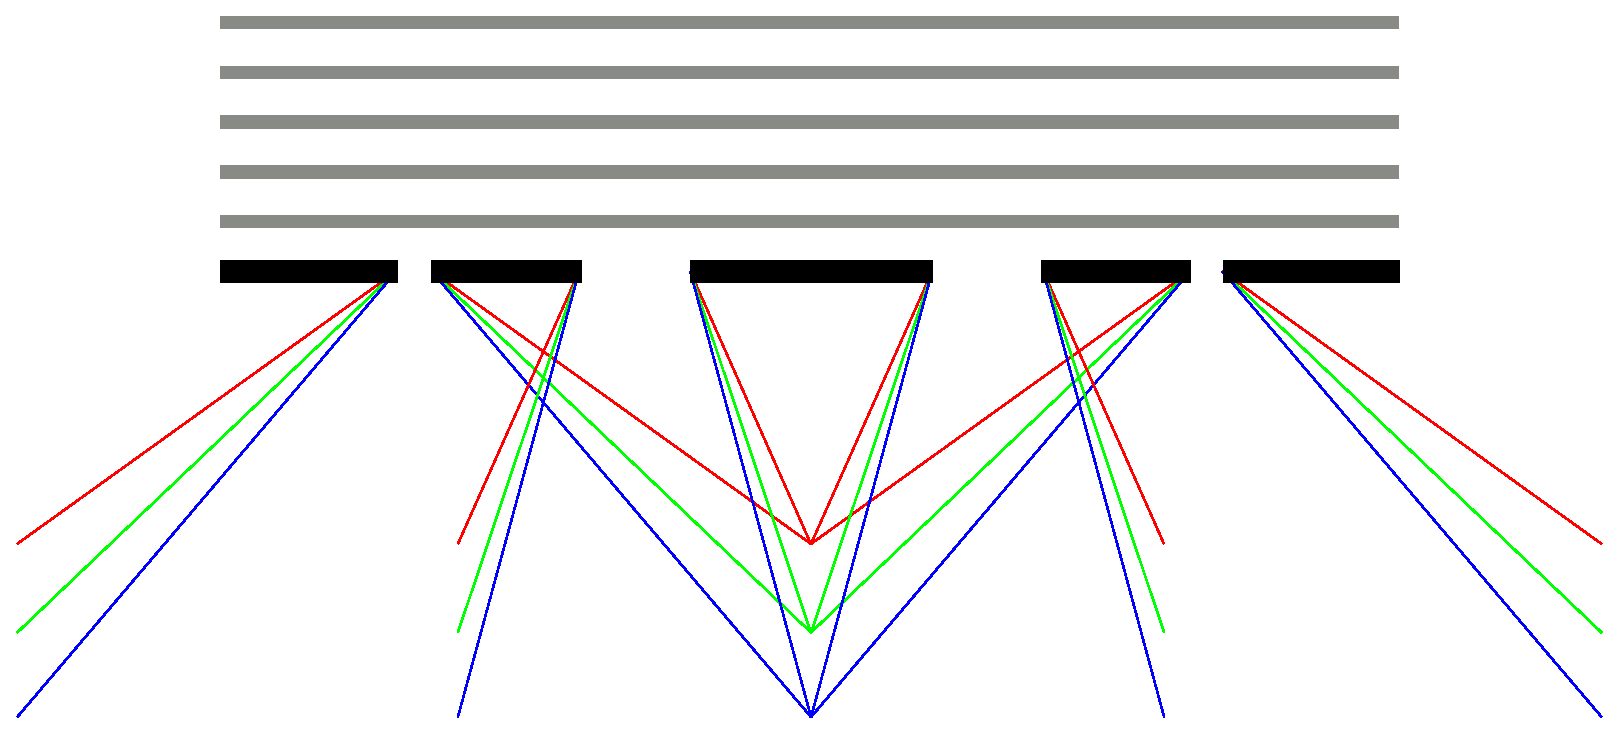
\includegraphics[width=4.0cm]{diffraction_ps_rgb}}
  \centerline{(a)}\medskip
\end{minipage}
\hfill
\begin{minipage}[b]{0.24\linewidth}
  \centering
  \centerline{
\includegraphics[width=2.0cm]{zoneplate}}
  \centerline{(b)}\medskip
\end{minipage}
\hfill
\begin{minipage}[b]{0.24\linewidth}
  \centering
  \centerline{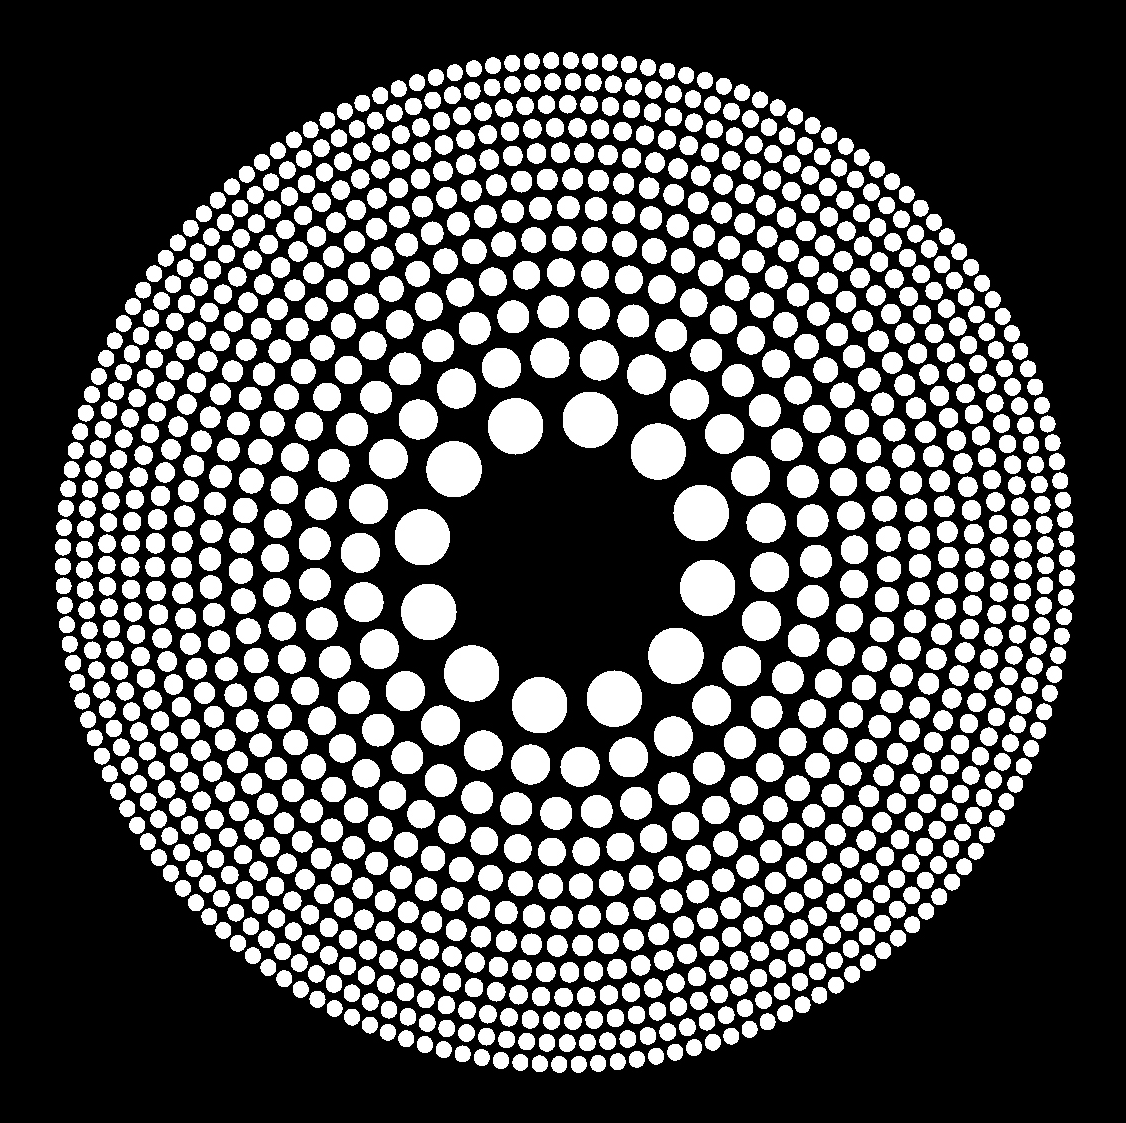
\includegraphics[width=2.0cm]{photonsieve}}
%  \vspace{1.5cm}
  \centerline{(c)}\medskip
\end{minipage}
\caption{(a) diffraction of a polychromatic wave through a diffractive lens (b) Fresnel zone
plate (c) photon sieve}
\label{fig:diff_lens}
%
\end{figure}

% FIXME
While diffraction produces a focused image of each source at separate planes, it
***.  This means that each measurement is actually a sum of all spectral
components of the source at varying degrees of focus.  An inverse problem
consisting of disentangling and deblurring of measurements must be solved in
order to recover the original source components.  Traditionally, measurement
locations are selected at the plane of focus for each spectral component.
However, as we show later in this paper, it is possible to improve on the
reconstruction quality in some situations by making measurements away from these
focal positions. We propose a greedy backward selection algorithm for
automatically discovering such a measurement configuration. Additionally, we
provide some bounds under which the greedy algorithm outperforms the traditional
selection approach.

% A different approach is to use a diffractive lens to perform spectral imaging.
% Diffractive lenses focus light using the diffraction principle. They have
% wavelength dependent focal length which is the property that enables them to be
% used as spectral imagers (see Figure \ref{fig:diff_lens}). Examples of
% diffractive lenses are Fresnel zone plates and their modifications (e.g. photon
% sieve) (see Figure \ref{fig:diff_lens}). Diffractive lenses are preferred in
% applications in UV and x-ray regimes where they can provide high resolution
% whereas reflective optics are very costly to manufacture to achieve high
% resolution and refractive lenses cannot be used due to light absorption in these
% regimes.


% Photon sieve spectral imaging (PSSI) is a modality that takes the advantage of
% the wavelength dependent focal length of a photon sieve to perform high
% resolution spectral imaging \cite{oktem2014icip}. It takes multiple exposures of
% the scene at different distances from the lens. Figure \ref{fig:pssi_drawing}
% illustrates the PSSI measurements for a scene radiating at two wavelengths
% $\lambda_1$ and $\lambda_2$. Each measurement consists of blurred superposition
% of the spectral images. The spectral images are then reconstructed from these
% measurements by solving a multi-frame deconvolution problem.


\begin{figure}[htb]
  \begin{minipage}[b]{1\linewidth}
    \centering
    \centerline{\includegraphics[width=8.5cm]{drawing}}
  \end{minipage}
  \caption{Imaging a scene with emissions at wavelengths $\lambda_1$ and
  $\lambda_2$. Measurements $y_1$ and $y_2$ are taken at two positions where one wavelength
  is in focus and the other is out of focus.}
  \label{fig:pssi_drawing}
\end{figure}

% Choice of measurement planes is an important factor affecting the reconstruction
% quality of the spectral images. Where to take measurements to maximize the
% fidelity of the reconstructions?

% One way is to scan the
% wavelength dimension by using color filters with narrow bandpass to filter
% desired wavelengths at each exposure. Another way is to capture the whole
% spectrum of a portion of the scene at an exposure, and scan a spatial dimension.
% In both methods, the 3D data-cube is then simply reconstructed by stacking the
% 2D measurements in the scanning dimension.

% There are also computational methods which rely on signal processing methods and
% computational power to improve upon the conventional methods in terms of spatial
% and spectral resolutions, total exposure time etc. They utilize more
% sophisticated image acquisition techniques than the conventional scanning-based
% methods, and computationally reconstruct the data-cube from multiplexed/encoded
% measurements. Such methods include compressive coded aperture snapshot spectral
% imaging (CASSI) [REF], compressive hyperspectral imaging by separable spectral
% and spatial operators (CHISS) [REF], and photon sieve spectral imaging (PSSI)
% \cite{oktem2014icip}.

% We will use PSSI as an example modality to explain and demonstrate our work
% because it  uses a diffractive lens, and it is a computational spectral imaging
% modality \cite{oktem2014icip}. Photon sieves, just like Fresnel zone plates, are
% diffractive lenses that use diffraction phenomenon to focus light. Diffractive
% lenses are preferred in applications in UV and x-ray regimes since they can
% provide high resolution whereas reflective optics are very costly to manufacture
% to achieve high resolution and refractive lenses cannot be used due to light
% absorption. They have wavelength dependent focal length which is what behind the
% working principle of PSSI. It takes multiple exposures at different distances
% from the lens to sample the measurement space.

\section{Forward Model and Statistical Formulation}
\label{sec:format}
In this section, we mathematically model a diffractive imaging system and
describe the process of recovering the spectral components. Consider a
polychromatic source that has $S$ two-dimensional spectral components $\bm{x}_1,
\dots, \bm{x}_S \in \mathbb R^{P \times P}$. Using a moving detector, we make
$M$ two-dimensional measurements $\bm{y}_1, \dots, \bm{y}_M \in \mathbb R^{P
\times P}$ at different distances from the lens.
% We allow for repeated measurements at the same plane for a more flexible model
% that can take into account non equal exposure times.
Due to linearity, each measurement is a superposition of blurred versions of the
$S$ sources. More formally,

\begin{equation}
\bm{y}_m = \sum_{s=1}^S \bm{h}_{m,s} \ast \bm{x}_s + \bm{n}_m
\label{eq:fwd_model}
\end{equation}

where $\bm{h}_{m,s}$ is a blurring kernel known as a \emph{point spread
function} (PSF), $\bm n_m \in \mathbb R^{P \times P}$ is the noise in the
measurements, and $\ast$ is a 2D convolution. Each PSF depends on the associated
source wavelength and measurement location and can be computed analytically. An
example set of PSF images for $M=S=2$ case is given in Figure \ref{fig:psfs}.
Since convolution is a linear operation, the relation in \eqref{eq:fwd_model}
can be written in matrix-vector notation as:

\begin{equation}
\begin{bmatrix}\vy_1 \\ \vdots \\ \vy_M\end{bmatrix}
=
\begin{bmatrix}
  \vA_{1, 1} & \hdots & \vA_{1, S} \\
  \vdots & & \vdots \\
  \vA_{M, 1} & \hdots & \vA_{M, S}
\end{bmatrix}
\begin{bmatrix}\vx_1 \\ \vdots \\ \vx_S\end{bmatrix}
+
\begin{bmatrix}\vn_1 \\ \vdots \\ \vn_M\end{bmatrix}
\label{eq:forward_mtx}
\end{equation}

where $\vy_m, \vx_s, \vn_m \in \mathbb R^{P^2}$ are the vectorized
versions of $\bm y_m, \bm x_s, \bm n_m$, and the measurement matrix $\vA
\in \mathbb R^{MP^2 \times SP^2}$ consists of the blocks $\vA_{m,s} \in \mathbb
R^{P^2 \times P^2}$ which correspond to the circular
convolution operation with the PSFs $\bm h_{m,s}$. Circular convolution
assumption allows for a computationally efficient algorithm using FFTs.

\begin{figure}[htb]
  \begin{minipage}[b]{1\linewidth}
    \centering
    \centerline{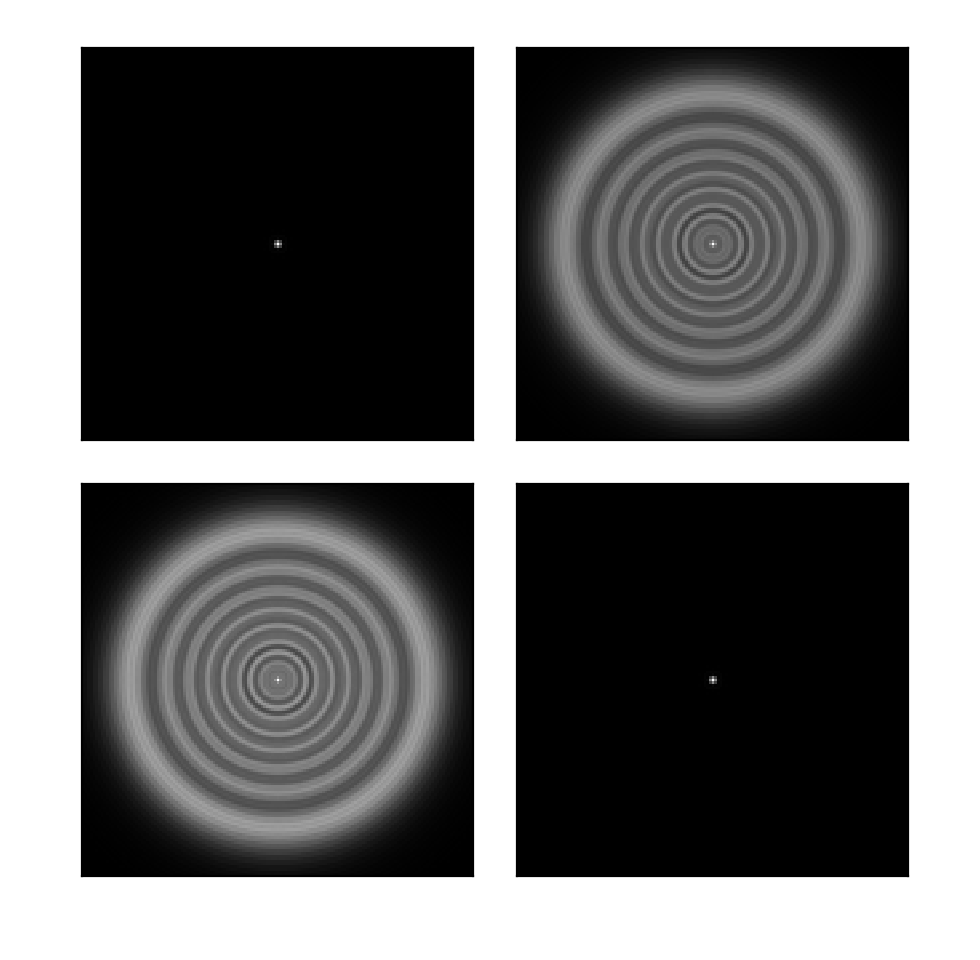
\includegraphics[width=5cm]{psfs}}
  \end{minipage}
  \caption{Example point spread functions for measuring a source with 2 spectral
    components at the focal planes of each component.}
  \label{fig:psfs}
\end{figure}

However, the problem of where to take measurements $\vy_1, \dots, \vy_M$ has not
been addressed and has an effect on the reconstruction quality.  In order to
compare the relative quality of different measurement configurations, it is
necessary to define some cost for the measurement matrix $\vA$.  A common cost
metric is the expected reconstruction error, or expected sum of squared errors
(SSE). However, we must have some strategy for the recovery of $\vx$ to get
reconstruction error and we must make statistical assumptions about $\vx$.
Maximum a posteriori (MAP) estimation is one such strategy.

We assume the original spectral components and noise are distributed according to a
normal distribution such that $\vx \sim \mathcal{N}(\vx_0, \Sigma_x)$ and
$\vn \sim \mathcal{N}(0, \Sigma_n)$.  The MAP estimate is then

% FIXME - dimensionality -> n
% use A instead of H?
$$
\begin{aligned}
  \hat{\vx}_{MAP} &= \argmax_{\vx} p(\vx | \vy)
  = \argmax_{\vx} p(\vy|\vx) p(\vx)\\
  &= \argmin_{\vx} \left[  - \log(p(\vy|\vx)) - \log
  p(\vx)\right] \\
  &= \vx_0 + \left( \vA^H\Sigma_{\vn}^{-1} \vA +
    \Sigma_{\vx}^{-1}\right)^{-1}
    \vA^H \Sigma_{\vn}^{-1} (\vy - \vA \vx_0)
\end{aligned}
$$
The reconstruction error is defined as $\ve = \vx - \vx_{\text{MAP}}$,
and the expected sum of squared error cost is $E[\norm{\ve}_2^2]$. This
expression can be rewritten in terms of the error covariance:

\begin{align*}
E[\norm{\ve}_2^2] =  E[\bm{e}^H\bm{e}] & = E[tr(\bm{e}^H\bm{e})] = E[tr(\bm{e}\bm{e}^H)] \\
& = tr(E[\bm{e}\bm{e}^H]) = tr(\bm{\Sigma_e})
\end{align*}

where the error covariance matrix is defined as $\bm{\Sigma_e} =
E[\bm{e}\bm{e^H}]$ and has the closed form expression:
\begin{equation}
\bm{\Sigma_e} = \left( \bm A^H\Sigma_{\bm{n}}^{-1} \bm A +
    \Sigma_{\bm{x}}^{-1}\right)^{-1}
\end{equation}
then our SSE cost becomes:
\begin{equation}
\text{Cost}(\bm{A}) = tr\left(\left( \bm A^H\Sigma_{\bm{n}}^{-1} \bm A +
    \Sigma_{\bm{x}}^{-1}\right)^{-1}\right)
\label{eq:sse-cost}
\end{equation}

\section{Measurement Selection Algorithm}
Having defined the cost metric, we are now looking for the best measurement
configuration to minimize the cost. Suppose we take $M$ measurements, each at
a distance $d_m$ from the lens for $m = 1, \dots, M$. 

\begin{equation}
\hat {\bm A} = \argmin_{\vA \in Q} \ \text{Cost}(\bm{A})
\label{eq:inverse}
\end{equation}

\begin{enumerate}
    \item inverse problem is simultaneous deblurring and disentanglement
    \item goal of paper is not to find optimal inversion strategy, but selection
          algorithm. will use tikhonov
    \item introduce MAP -> tikhonov
    \item model assumptions, gaussian X, gaussian Noise
      \item with this framework, how do we choose where to make measurements to
        get the best reconstruction quality? what distances from lens?
        \item in the next section, we introduce an cost metric to help minimize
          reconstruction error and propose an algorithm for minimizing this metric.
\end{enumerate}

\begin{enumerate}
  \item introduce sse.  now have a method for comparing two measurement
    configurations for which gives better reconstruction
  \item motivate that searching for optimal measurement configuration is
    infeasible.  show complexity.  suffers from dimensionality problem. for a realistic situation (e.g. 3 spectral
    components, 10 candidate positions, 5 measurements). its a huge number.
  \item known as subset selection problem
  \item one common approach is greedy hill climbing, which iteratively finds
    a solution by making temporary, incremental changes to the currently
    selected subset before making a change. commonly this is applied to rows
    of a matrix to find optimal configuration
  \item sharif paper introduces clustered sequential backward selection
    algorithm.  backward because we start with many potential candidate locations and eliminate.
    clustered because eliminating a measurement candidate eliminates
    multiple rows from the matrix H.
    \item $d_1, \dots, d_C$  $n_1, \dots, n_C$  $\sum_{c=1}^C n_c = M$
\end{enumerate}


\section{Reconstruction Results}

\subsection{Subheadings}

\subsubsection{Sub-subheadings}

\section{Bounds}

\section{PAGE NUMBERING}

\section{ILLUSTRATIONS, GRAPHS, AND PHOTOGRAPHS}

% Below is an example of how to insert images. Delete the ``\vspace'' line,
% uncomment the preceding line ``\centerline...'' and replace ``imageX.ps''
% with a suitable PostScript file name.
% -------------------------------------------------------------------------


\vfill\pagebreak

\section{REFERENCES}
\label{sec:refs}


% References should be produced using the bibtex program from suitable
% BiBTeX files (here: strings, refs, manuals). The IEEEbib.bst bibliography
% style file from IEEE produces unsorted bibliography list.
% -------------------------------------------------------------------------
\bibliographystyle{IEEEbib}
\bibliography{bibliography}

\end{document}
